\chapter{Evaluation}

In this chapter, we will evaluate our proposed planning model based on reinforcement learning and attention mechanism \ref{vrptw-model}.

\section{Dataset}
The dataset used for training and evaluation was generated on the fly via a uniform probability distribution within a given range. The reason we decided to generate the data is that learning reinforcement policy requires a large amount of training data. Since it learns by interacting with the environment, we do not need labeled datasets and generating them seems as the best approach. Nevertheless, in further work, the model will require other kinds of distribution to simulate a real-world demand.

In real-world routing applications, the geographic coordinate system is typically used for specifying locations. However, our proposed model requires locations between $[0, 1]$ to achieve model convergence. The locations of depots and delivery nodes were generated via uniform distribution within a range of $[0, 1] \times [0, 1]$.

The data for the demand capacity of a delivery node is a discrete number $\{1, \cdots, 9\}$ chosen uniformly at random with assumption that the depot has a demand capacity of zero. 

Lastly, each location has assigned time windows that work as a soft constraint at which time a vehicle is supposed to visit the node. We generate different lengths of time windows based on the problem size (20, 50, 100). For the problem size of 20 nodes, the time window value occurs in a range of $\{0, \cdots, 10\}$ with the condition that the length of the time window is less than four. The problem size of 50 nodes has the upper bound set to 20 with a maximal length of 6 and the case of 100 nodes, the upper bound is 40 and the maximal window length is 9. Similarly, the start and end of a time window are generated with uniform distribution.

\section{Sample Solutions}
To better imagine the complexity and variability of solving \gls{vrptw}, in Figure \ref{fig:sample-plan} we illustrate a random solution predicted by our \gls{ai} model.

\begin{figure}[ht]
    \centering
    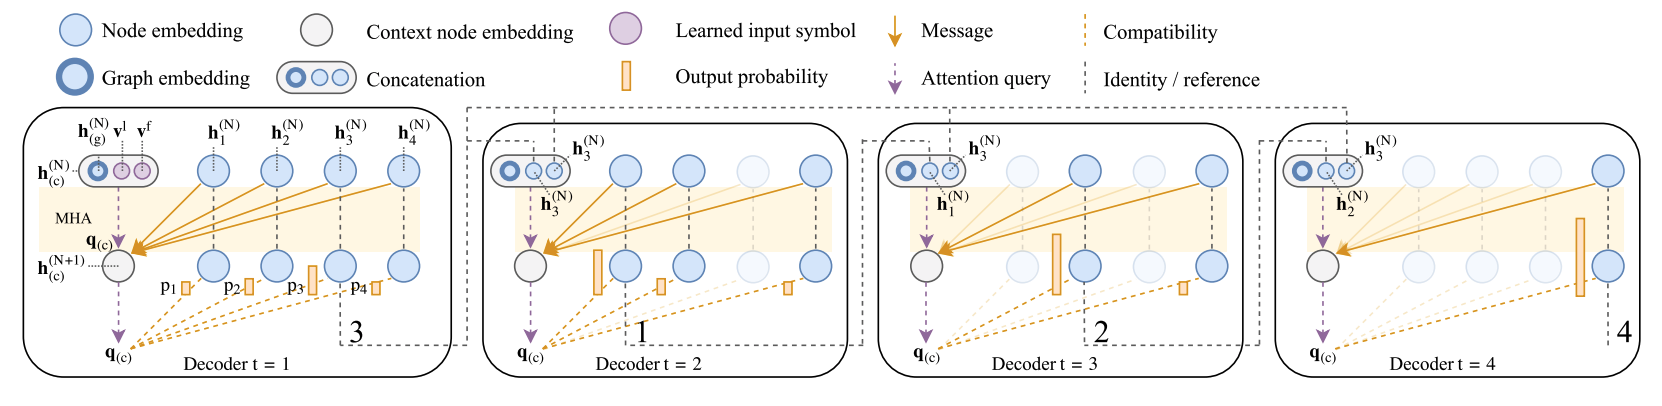
\includegraphics[width=1.0\textwidth]{resources/vrptw-ai/decoder-diagram.png}
    \caption{TODO \cite{attention-route}}
    \label{fig:encoder-diagram}
\end{figure}

The \gls{ai} model has to optimize the route path with focus to minimize the travelled distance, but simultaneously early and arrivals should be avoided. We may see in Figure \ref{fig:sample-plan} that model has successfully learned the policy how to pick the next node to visit, the time windows are almost cascadingly sorted, and the routes are optimized based on distance. 

It is clearly not an optimal solution, but it proves that the problem of vehicle routing with time windows is  possible to be solved with \gls{ml} and the research is on the right path to do so. In the next section \ref{benchmarking} we compare the model with other optimization and heuristics methods.

\section{Experiments}
\subsection{Time Windows}
The main goal of this thesis was to integrate the constraint of time windows to \gls{vrp} model introduced by Kool et al. \cite{attention-route}. The model is extended by our proposed cost function \ref{vrptw-cost} that penalizes early and late arrivals. The early arrival is not as crucial as delayed visit, so we have decided that the penalty for early arrival is always less than late visit $p_e < p_l$.

Finding a proper penalty values is one of the most important steps because an incorrect penalty highly influences the model in choosing the next node to visit. We have empirically tested various kinds of penalties
and updated them based on our observations.

We have observed if 
\begin{figure}[ht]
    \centering
    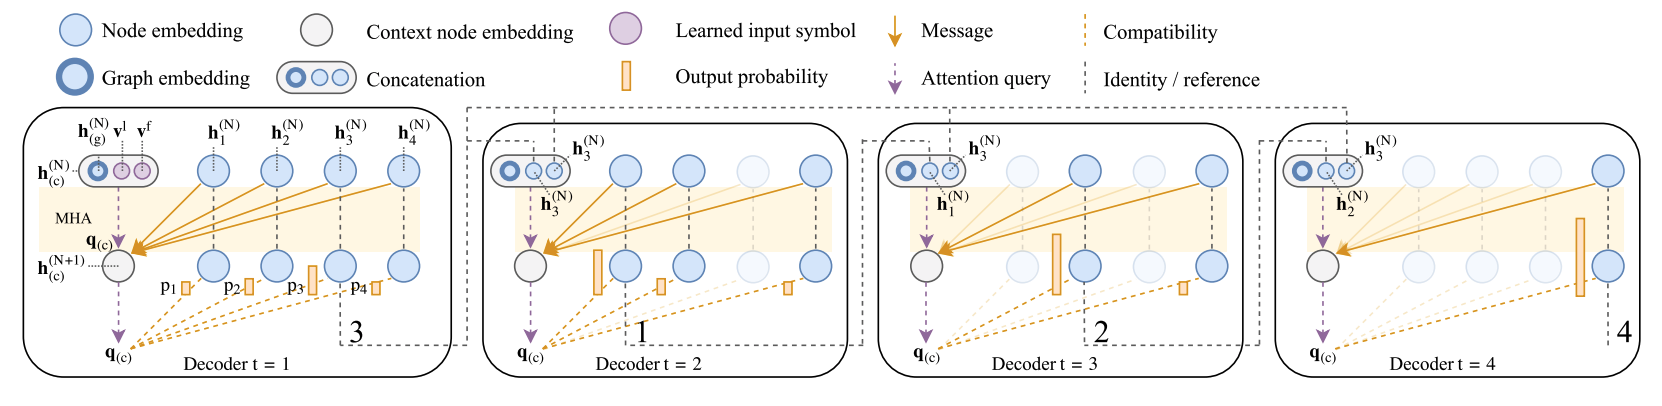
\includegraphics[width=1.0\textwidth]{resources/vrptw-ai/decoder-diagram.png}
    \caption{TODO \cite{attention-route}}
    \label{fig:encoder-diagram}
\end{figure}

\subsection{Balancing Plans}
In real-world solution of \gls{vrp}, we aim to balance the size of the delivery plan across vehicles so the number of nodes in a given route is uniformly distributed. However, we have noticed that the model was additional routes of size one or two nodes as illustrated on Figure \ref{fig:unbalanced}.

\begin{figure}[ht]
    \centering
    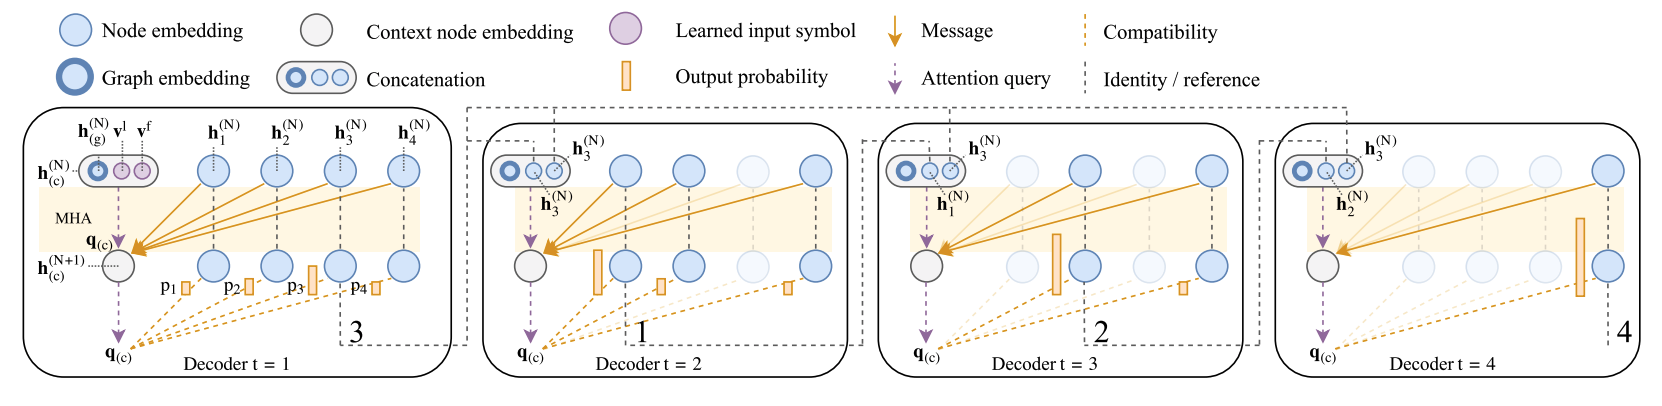
\includegraphics[width=1.0\textwidth]{resources/vrptw-ai/decoder-diagram.png}
    \caption{Unbalanced delivery plans \cite{attention-route}}
    \label{fig:unbalanced}
\end{figure}

Therefore, we have decided to penalize the delivery plans that are not balanced by including an unbalance penalty. This calcultes a standard divation of plans. This approach helped in creating balanced delivery plans.

\begin{figure}[ht]
    \centering
    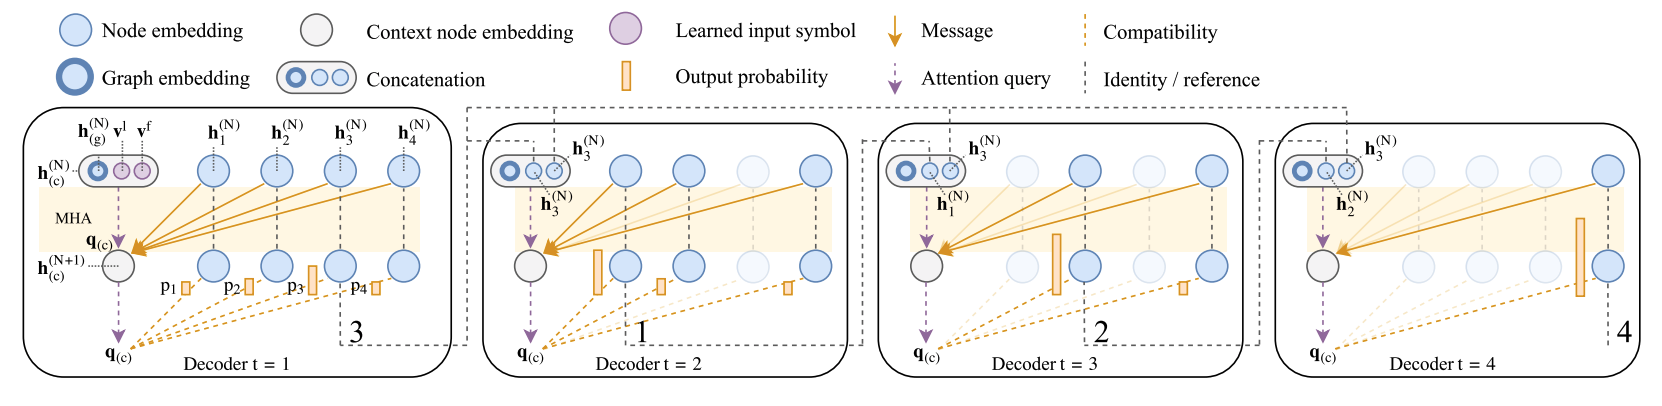
\includegraphics[width=1.0\textwidth]{resources/vrptw-ai/decoder-diagram.png}
    \caption{Balanced delivery plans \cite{attention-route}}
    \label{fig:balanced}
\end{figure}

\subsection{Generalization}

Downside of this model that it is sensitive on data input and has a poor generalization. If you introduce a data which have not seen before it is not possible to create delivery plans and just sands to each node a one vehicle \ref{fig:model-breaks}.

\begin{figure}[ht]
    \centering
    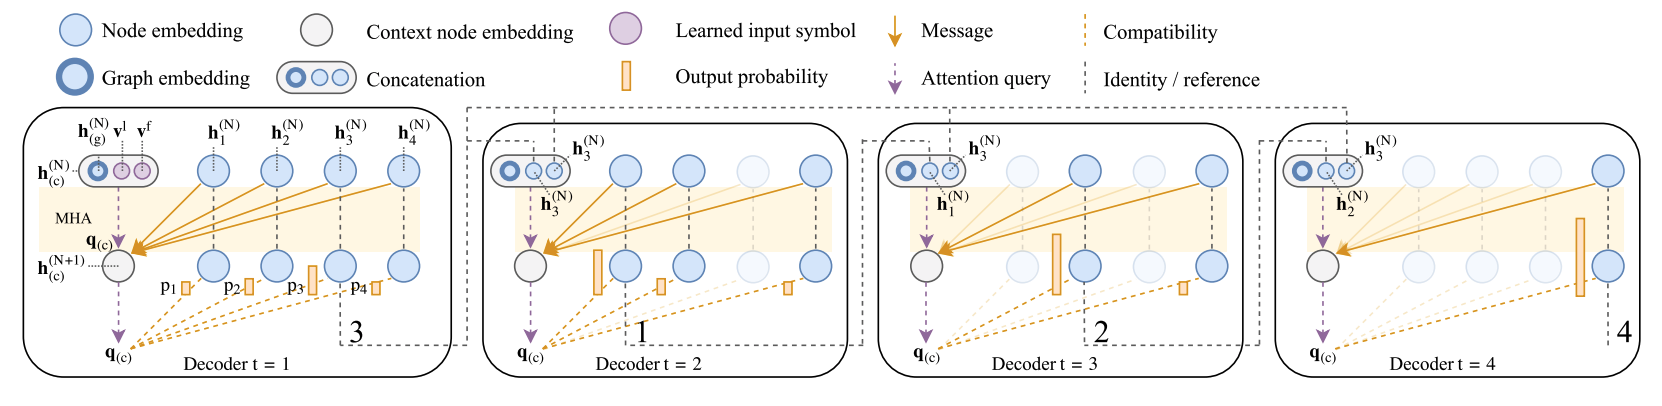
\includegraphics[width=1.0\textwidth]{resources/vrptw-ai/decoder-diagram.png}
    \caption{Sensitive on data input}
    \label{fig:model-breaks}
\end{figure}

Additionaly, it is also sensitive on problem size. If you train the network on problems of 20 nodes, the perfromance is continously degranding with problem instance. We tried training the model on dataset of  different problem sizes and the network was not effectbvily learning. The model just overfits on given problem size. 

Solution for the different problem size is to train multiple models for each problem size and pro given instance chose the proper one. 

\subsection{Training Process}

Experimenting with different values of network hyperparameters has not been done in this thesis. We only focused on proving if even such a problem like \gls{vrptw} can be sub-optimally solved via neural networks. We have used the same hyperparameters as Kool et al. \cite{attention-route} in their research.

The training of such a network is extremly time consuming and requires 

\section{Benchmarking}
The \gls{ml} model for sub-optimally solving \gls{vrptw} instances can predict a feasible solution, but in order to evaluate the model performance, we need to compare it with other reliable methods. 

The first benchmark is insertion heuristics \ref{insertion-heuristics} which produces a feasible solution in a matter of seconds. It is frequently used to generate an initial solution which is then optimized by a local search algorithm. The second typical benchmark used in research papers is OR-Tools framework \ref{or-tools} is widely used for many optimization tasks. Lastly, the third benchmark combines insertion heuristics as an initial solution and OR-Tools planner to optimize it.

\begin{table}[ht]
\centering
\resizebox{\textwidth}{!}{

\begin{tabular}{rrrrrrrrrrrrrr}
\toprule
distance\_cost & \multicolumn{2}{l}{delay\_cost} & \multicolumn{2}{l}{earliness\_cost} & \multicolumn{2}{l}{sum\_duration\_cost} & \multicolumn{2}{l}{delivery\_expense\_cost} & \multicolumn{3}{l}{num\_couriers} & computation\_time \\
         mean &        std &       mean &       std &           mean &        std &              mean &        std &                  mean &          std &         mean & min & max &             mean \\
  1000.702461 & 126.790309 &   0.000000 &  0.000000 &     838.389844 &  87.218392 &       1653.238802 & 271.664752 &         333649.859375 & 54394.085587 &     3.000000 &   3 &   3 &         1.127346 \\
\midrule
   473.614450 &  53.948290 &   2.858073 &  6.681443 &     846.664062 & 138.443196 &       1234.803646 & 261.313242 &         248381.593750 & 52287.538762 &     3.000000 &   3 &   3 &       119.783904 \\
   476.834627 &  52.003944 &   1.336458 &  2.423643 &     817.094010 & 137.903342 &       1248.783333 & 334.401754 &         251187.234375 & 66897.706961 &     3.000000 &   3 &   3 &       120.840771 \\
   472.984988 &  52.507476 &   2.606771 &  6.541328 &     846.213802 & 139.405468 &       1227.716406 & 261.011829 &         246962.250000 & 52222.412802 &     3.000000 &   3 &   3 &       120.002144 \\
   613.744970 &  85.309954 &  40.472135 & 26.160495 &     872.414323 & 135.223670 &       1533.759115 & 330.666886 &         308592.984375 & 66175.534588 &     1.140625 &   1 &   3 &         0.177940 \\
\bottomrule
\end{tabular}

}
\caption{Paired t-test of most common TF families for Pearson Correlations} 
\end{table} 

